\subsection{Ľavicová halda} 
\paragraph{Popis.}
V ľavicovej halde si pre každý vrchol pamätáme hodnotu \emph{rank}, čo je najkratšia 
vzdialenosť vrcholu k \emph{externému vrcholu}. Každému vrcholu haldy, ktorému chýba aspoň jeden syn, sú 
doplnené špeciálne vrcholy tak, aby mal každý vrchol oboch synov. Týmto špeciálnym vrcholom hovoríme externé 
a nie sú súčasťou haldy. Ich rank je $0$. Rank vrcholu $x$ je daný rekurzívne ako $rank(x) 
= 1 + min\{rank(left(x)), rank(right(x)) \}$. Pre ľavicovú haldu špeciálne platí, že rank pravého syna je menší 
alebo rovný ako rank ľavého syna. Toto zabezpečuje pre každý podstrom, že pravá cesta je vždy kratšia 
ako ľavá cesta.

\paragraph{Operácie.}
Najdôležitejšia operácia vykonávaná na Ľavicovej halde je \emph{meld($i$,$j$)}. Pomocou nej si zadefinujeme aj \emph{insert($x$)} a 
\emph{deleteMin}. Haldy sa spájajú pozdĺž pravej cesty. Postupne prechádzame odvrchu nadol celú pravú cestu haldy $i$ a 
porovnávame kľúče s koreňom haldy $j$. Ak narazíme na kľúč vrcholu $v$ v halde $i$, ktorý je väčší ako kľúč v koreni 
$w$ haldy $j$, vrcholy vymeníme. Teda z $w$ sa stane pravý syn otca $v$ a z $v$ sa stane halda $j$. Kľúč prázdnej 
haldy považujeme za nekonečno. Takto pokračujeme, až kým nedôjdeme na koniec pravej cesty haldy $i$.
Potom nasleduje fáza úpravy rankov. Ranky sa mohli zmeniť len na pravej, spájacej ceste, preto ich pozdĺž tejto cesty 
zdola nahor upravíme.
Nakoniec pre ľavicovú haldu musí byť dodržané pravidlo o veľkosti rankov synov. Preto opäť prejdeme pravú cestu 
výslednej haldy a pokiaľ je niekde pravidlo porušené, bratov vymeníme.\footnote{Druhý a tretí krok sa dajú robiť 
súčasne, avšak z hľadiska prehľadnosti vizualizácie sú v našom programe implementované po sebe.}

\begin{figure}
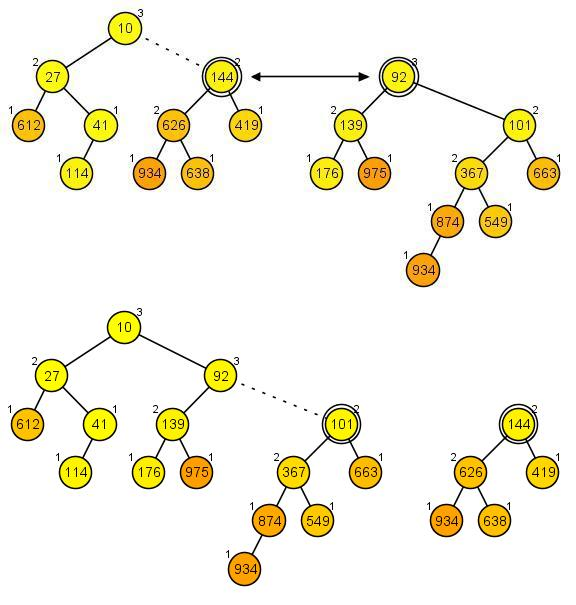
\includegraphics[width=\columnwidth]{obrazky/leftistmeld.png}
\caption{\emph{} 
Spájanie pozdĺž pravej cesty} 
\label{img:leftmeld} 
\end{figure}

Pokiaľ máme definovanú operáciu \emph{meld($i$,$j$)}, zadefinovať \emph{insert($x$)} na halde $i$ je jednoduché. Vytvorí sa nová jednoprvková halda $j$ obsahujúca iba vrchol $x$ a zavolá sa \emph{meld($i$,$j$)}.

Operácia \emph{deleteMin} najprv vymaže vrchol haldy $h$ a potom zavolá \emph{meld(left($h$), right($h$))}.

Hoci operácia \emph{decreaseKey} nie je štandardná pre Ľavicovú haldu, v programe je definovaná ako \emph{decreaseKey} pre 
binárnu haldu. Teda po znížení kľúča vrchol "prebubláva" nahor.

\paragraph{Časová zložitosť.}
Veľkým plusom ľavicovej haldy je časová zložitosť pre spájanie $log(n)$, kde $n$ je súčet vrcholov oboch háld, 
ktoré spájame. Toto sa dosiahne vďaka tomu, že cesta, pozdĺž ktorej sa dve haldy spájajú, sa udržuje čo 
najkratšia. \emph{Insert(x)} a \emph{deleteMin} sa majú rovnakú zložitosť ako \emph{meld(i,j)}. \emph{CreateHeap} a \emph{findMin} majú konštantnú časovú zložitosť.
Existuje lazy verzia Ľavicovej haldy (\cite{left}), ktorá odkladá vymazávanie a spájanie. Časová zložitosť týchto dvoch 
operácií sa stane konšatntnou, na úkor operácie \emph{findMin}. Tento druh sme však neimplementovali, preto sa ním 
nebudeme zaoberať.